\documentclass[10pt,a4paper]{article}
\usepackage[utf8]{inputenc}
\usepackage[T1]{fontenc}
\usepackage{amsmath}
\usepackage{amssymb}
\usepackage{graphicx}

\usepackage{pgfplots}
\begin{document}
	\begin{figure}
		\centering
		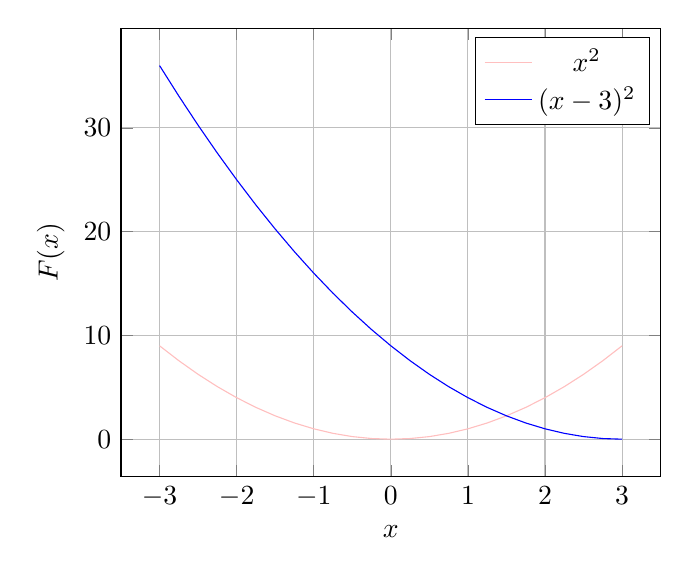
\begin{tikzpicture}
			\begin{axis}
				[xmin=-3.5,xmax=3.5,
				xlabel=\(x\),
				ylabel=\(F(x)\),
				grid=both
				]
				\addplot[domain=-3:3,color=pink]{x^2};
				\addplot[domain=-3:3,color=blue]{(x-3)^2};
				\legend{\(x^2\), \((x-3)^2\)};
			\end{axis}
		\end{tikzpicture}
		\caption{A simple Graph}
	\end{figure}
	
\end{document}